\begingroup
	\pgfdeclarelayer{background layer}
	\pgfsetlayers{background layer,main}
	\tikzstyle{zero}=[circle,draw=black,fill=white,inner sep=0pt,minimum size=2.5mm]
	\tikzstyle{one}=[circle,draw=black,fill=black,inner sep=0pt,minimum size=2.5mm]
	\tikzstyle{two}=[circle,draw=black,fill=gray,inner sep=0pt,minimum size=2.5mm]
		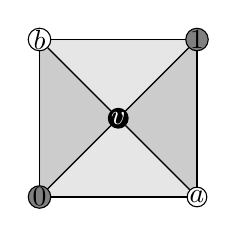
\begin{tikzpicture}
			\node (1) at (-1,-1) [two] {$0$};
			\node (a) at (1,-1) [zero] {$a$};
			\node (0) at (1,1) [two] {$1$};
			\node (b) at (-1,1) [zero] {$b$};
			\node [white] (x) at (0,0) [one] {$v$};
			
			\draw (1) -- (a);
			\draw (1) -- (b);
			\draw (a) -- (0);
			\draw (b) -- (0);
			
			\draw (x) -- (a);
			\draw (1) -- (x);
			\draw (x) -- (0);
			\draw (b) -- (x);
			
			\begin{pgfonlayer}{background layer}
				\filldraw [gray,opacity=0.2] (-1,1)--(1,1)--(0,0)--(-1,1);
				\filldraw [gray,opacity=0.2] (-1,-1)--(1,-1)--(0,0)--(-1,-1);
				\filldraw [black,opacity=0.2] (-1,-1)--(-1,1)--(0,0)--(-1,-1);
				\filldraw [black,opacity=0.2] (1,-1)--(1,1)--(0,0)--(1,-1);
			\end{pgfonlayer}			
		\end{tikzpicture}
%	\label{fig:eg_cone_k_2_2}	
\endgroup